\documentclass[report]{subfiles}
\begin{document}
    \chapter{METHODOLOGY}
    \section{Flowchart}
    \begin{figure}[H]
        \centering
        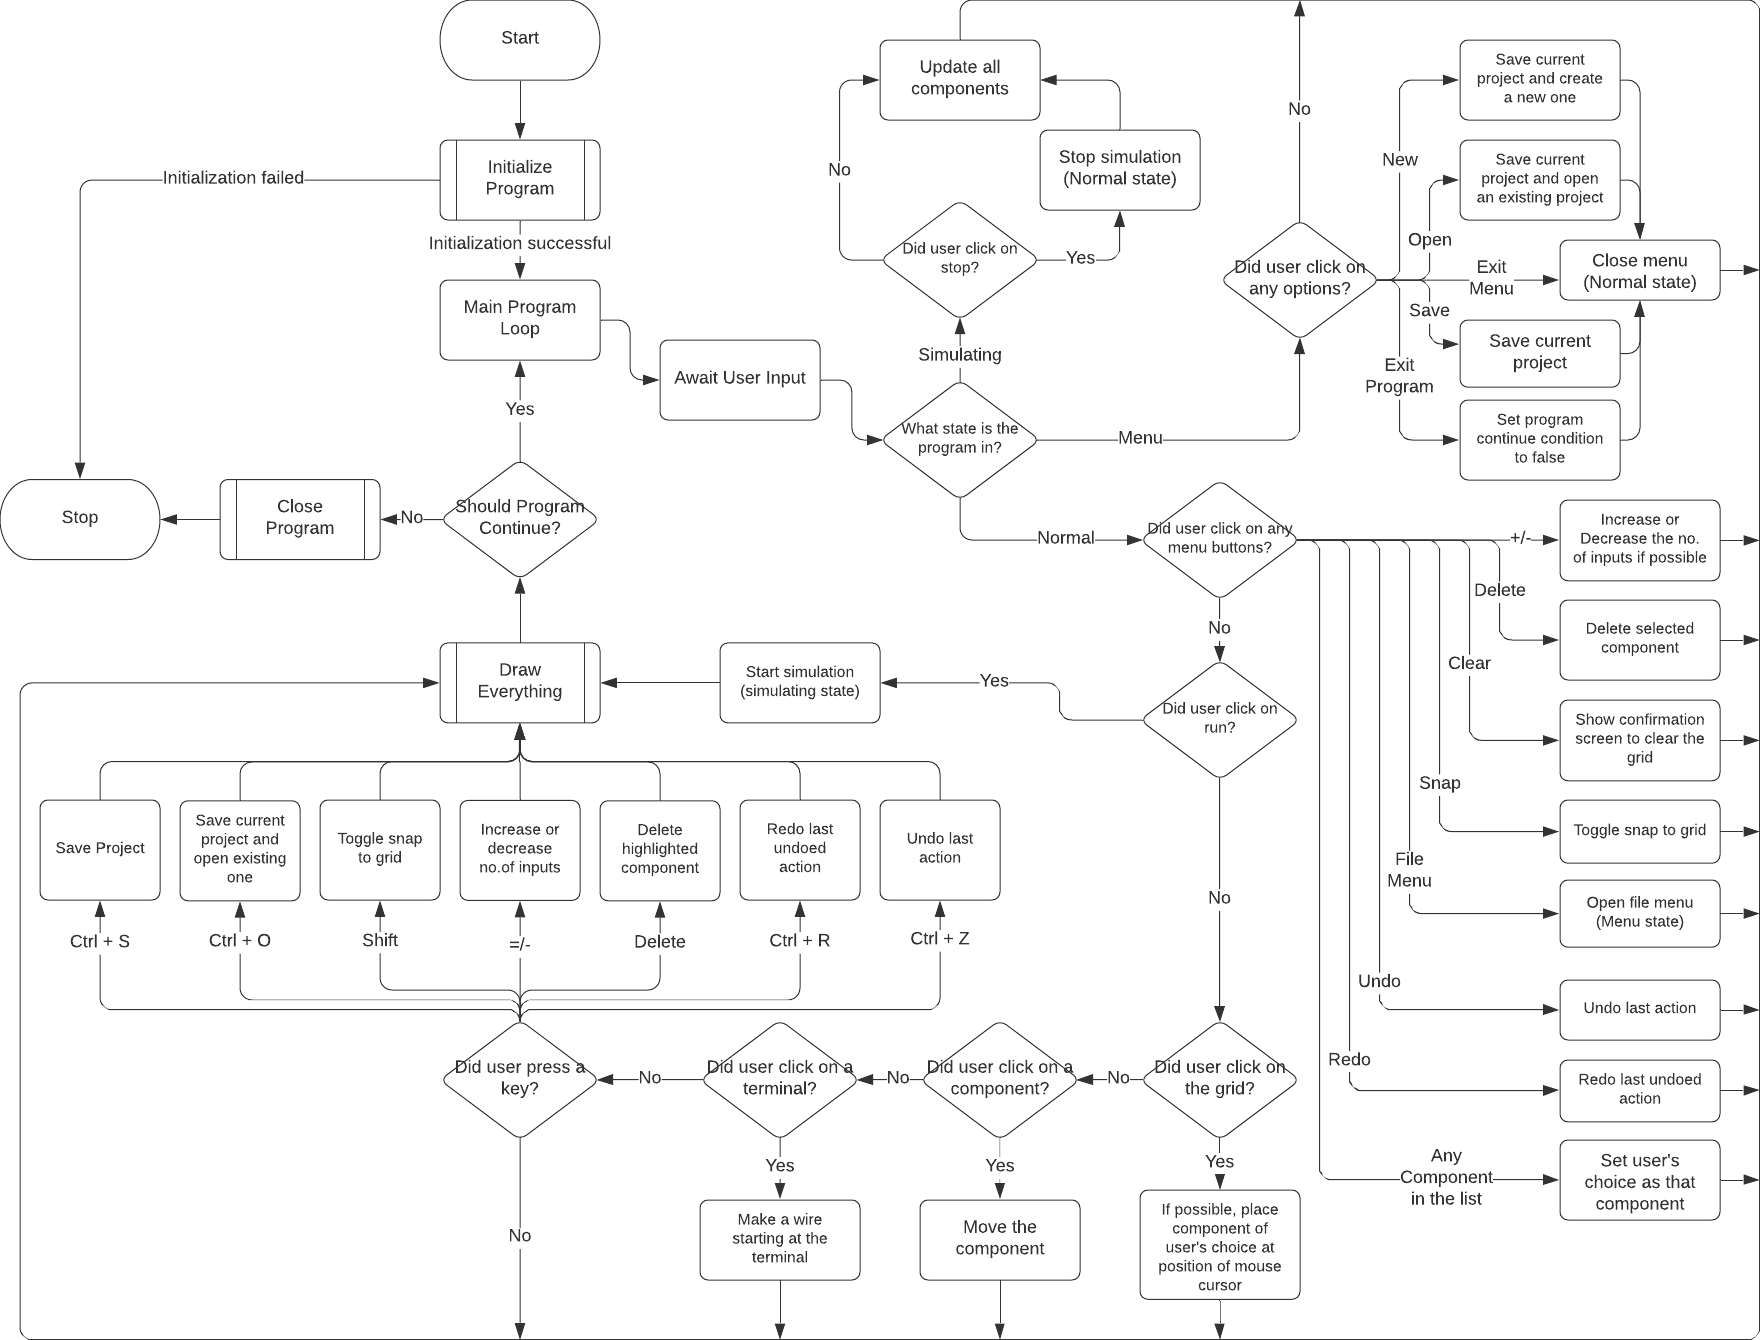
\includegraphics[width=\textwidth]{../graphics/Flowchart.png}
        \caption{Flowchart of the program}
    \end{figure}
    \newpage
    \section{Working of the program}
    Working of the program can be described in the following three steps: 
    \subsection{Initialize}
    When the program is launched, initialization is carried out. If initialization is unsucessful, the program will display and error and quit. During this process, the libraries used by the program (SDL2 and SDL2\_ttf) are initialized. Then the SDL window and renderer are created. Fonts used to display text in the program are loaded and then a character map is created using the fonts. Since SDL2\_ttf ant the fonts are no longer required after the character map has been created, the fonts get closed and SDL2\_ttf is quit.\\
        \textbf{\texttt{Algorithm for Inititalizing}}
        \begin{verbatim}
initialize SDL
did SDL initialize successfully?
  yes: continue
  no : display error
     exit program
create SDL window
create SDL renderer
were the window and renderer created successfully?
  yes: continue
  no: display error
    exit program
initialize the grid
  fill grid with -1
had user clicked on a file to open?
  read from file and update grid
  update window title
initialize menu
  set dimensions and positions for all buttons
change directory to directory of executable 
initialize SDL_ttf
did SDL_ttf initialize successfully?
  yes: continue
  no : display error
       exit program
load fonts
were fonts loaded successfully?
  yes: continue
  no : display error
       exit program
create character map
  create textures for all characters to be used
close fonts
close SDL_ttf
        \end{verbatim}
    \subsection{Loop}
    All user interaction, simulation and rendering happen inside the main program loop. During each iteration of the loop, the program waits for user input and then processes it as shown in the flowchart. Then all components of the program are rendered (drawn) onto the screen. If the simulation is running then all the components get updated. The loop continues to run until the user quits (presses the X button in title bar or presses Alt+F4) or exits program from the menu.\\
        \textbf{\texttt{Algorithm for Loop}}
        \begin{verbatim}
loop if program continue condition is true{
  await user input
  what state is program in?
    normal:
      if user clicked on RUN
        start simulation
      if user clicked on + or user pressed = key
        increase no. of inputs of current choice if possible
      if user clicked on - or user pressed - key
        decrease no. of inputs of current choice if possible
      if user clicked on Undo or user pressed Ctrl + z
        undo last action
      if user clicked on Redo or user pressed Ctrl + r
        redo last undoed action
      if user clicked on Delete Component or user pressed Delete key
        delete selected component on the grid
      if user clicked on Clear Grid
        show confirmation screen
          user clicked yes: empty the grid
      if user clicked on Snap to Grid or user held Shift
        toggle snapping to grid
        is snapping toggled on?
          yes: set snap button text to "Snap to Grid: On"
          no : set snap button text to "Snap to Grid: Off"
      if user clicked on File Menu
        open the menu
      if user clicked on any component in the list
        set user's choice to be that component
      if user pressed Ctrl + o
        save current project and open existing one
      if user pressed Ctrl + s
        save project
      if user clicked on component on the grid
        move the component
      if user clicked on terminal
        make wire starting at that terminal
      if user clicked on the grid
        if possible place user's choice of component on the grid
        at current mouse cursor position
    simulating:
      if user clicked on STOP
        stop simulation
      update all components
    menu:
      if user clicked on Save:
        save current project
        close menu
      if user clicked on New:
        save current project and create a new one
        close menu
      if user clicked on Open:
        save current project and open an existing one
        close menu
      if user clicked on Exit Menu:
        close menu
      if user clicked on Exit Program:
        set program continue condition to false 
        close menu
  draw everything
    draw menu
    draw grid
    draw components
    draw wires
}
        \end{verbatim}
    \subsection{Close}
    After the program exits from the loop, it calls some clean up functions which destroy the textures, window and renderer, and free memory.\\
        \textbf{\texttt{Algorithm for Closing}}
        \begin{verbatim}
destroy all textures
destroy window
destroy renderer
quit SDL
exit program
        \end{verbatim}
    \section{Brief Descriptions of the source files}
        \subsection{component.c and component.h}
    As the name suggests, these files contain all the necessary
    information about the components used in the program. The header
    file defines a structure named Component that encompasses the
    details about a component including its size, position, input source,
    number of inputs, input state(s), output state(s) and other
    information which is later used.
    The output of any component (except clock and state) depends on
    its input(s). To get the desired output for any component from its
    inputs, the source file defines different component specific
    functions. The working of these functions is pretty straight-forward
    as they follow the standard logic operations available in C. As for
    the clock, its output is generated based on the value of time
    variable, which changes as the program progresses, defined in
    program.c. The clock inverts its current state when time reaches a
    certain value. The output of state is inverted when the user clicks
    on it.
\subsection{draw.h and draw.c}
    These two files contain the variables and functions that are
    responsible for drawing all the elements that are visible on the
    screen such as Buttons, Components, and Wires. It also handles
    rendering text in the SDL window where necessary. The header
    file defines an enumeration of confirmation flags that are later used
    to ask the user for confirmation on certain operations.
    The standard rendering functions available in the SDL library are
    used in order to draw Buttons and Components. However, SDL
    does not offer the functionality to draw curves. So, a simple
    algorithm that approximates a cubic Bezier Curve is used to draw
    wires.
    As for displaying text, a character map consisting of all the ASCII
    characters is predefined when the program starts. The font used is
    robotoo.ttf. The character map is later used to display any text
    (ASCII based) on the screen.
\subsection{interaction.h and interaction.c}
    User interaction is an integral part of any program, even more so
    for programs that use both mouse and keyboard to take input.
    These two files are responsible for handling such interactions. The
    header file defines various structures that are necessary for the
    Undo/Redo functionalities.
    The source file defines different functions that determine what will
    happen when a certain button is pressed or when a component is
    placed on the grid. Since these functions handle interaction with
    the user, they are usually only called when an event occurs. An
    SDL event encompasses mouse clicks, keyboard presses, etc.
    Different functions are called for different events. This
    coordination is handled in the file program.c.
\subsection{program.h and program.c}
    To keep the main.c file clean, the main program loop is defined in
    this file. For this reason, it acts as the centerpiece of the program
    that coordinates the functions of all other files. To begin with, the
    header file defines macros for configuring the main window and
    different elements inside it. Also, the colors that are frequently
    used in the program are defined here.
    The source file can be vaguely divided into two parts:
    Initialization and Main Program Loop. The initialization part is
    responsible for setting up all the necessary elements needed for the
    program to function properly. This is a one-time process that
    occurs when the program is launched.
    The Main Program Loop, as the name suggests, is a loop that runs
    over and over until the user exits the program. Everything that the
    user does inside the program is handled in this section. During
    each loop, the program checks for events, performs necessary
    operations based on them, updates the elements on the screen if
    required, and redraws all of those elements.
\subsection{main.c}
    As mentioned earlier, this file is kept as clean as possible by
    defining the main loop in program.c. The main function calls functions for initialization, the main
    program loop, and finally closing the program.
\end{document}
